% Plan (~10 pages).
\chapter{Results}

% Plan: ~1 page.
\section{Simulation Outputs}

\Cref{fig:simulation-gaussian-evolution} shows the field amplitude at the start and end of a
simulation with a Gaussian input pulse and group-velocity dispersion enabled. The pulse
broadens during propagation, while its peak amplitude decreases. This is the expected change
for a dispersive pulse and provides a simple example of the field output produced by the
simulation.

\begin{figure}
  \centering
  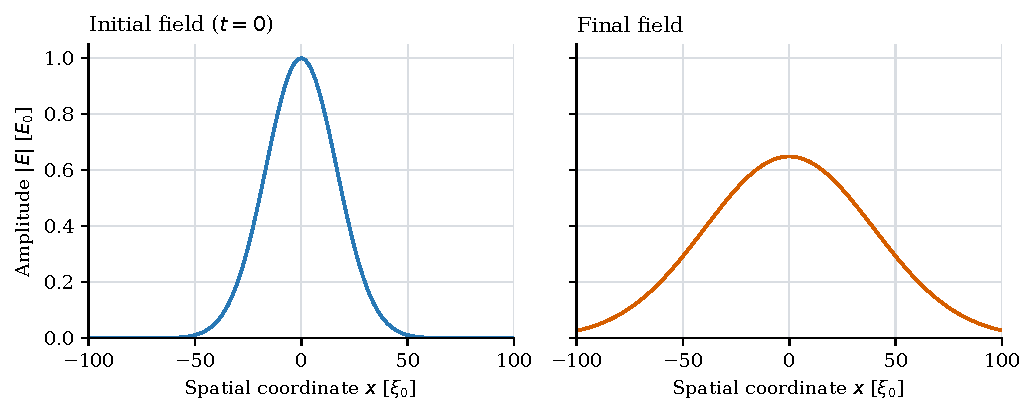
\includegraphics[width=\textwidth]{simulation_gaussian_evolution}
  \caption{Initial and final field amplitudes for the built-in Gaussian channel in a
  group-velocity-dispersion simulation. Both panels show the same spatial range,
  $-100 \leq x/\xi_0 \leq 100$. The final pulse is broader and has a lower peak amplitude.}
  \label{fig:simulation-gaussian-evolution}
\end{figure}

As discussed earlier, the simulation now allows for custom defined pulse shapes. An example
of this can be seen below in \Cref{fig:simulation-builtin-custom} which shoes the pre and post 
simulation of these shapes. For this example, the custom amplitude profile is
\(\exp(-x^2/50)(1 + 0.5\cos(x))\), the same as seen in \Cref{fig:custom-functions}.
The two profiles are launched as separate forward channels in the same simulation,
illustrating that a custom shape can be used alongside a preset shape.

\begin{figure}
  \centering
  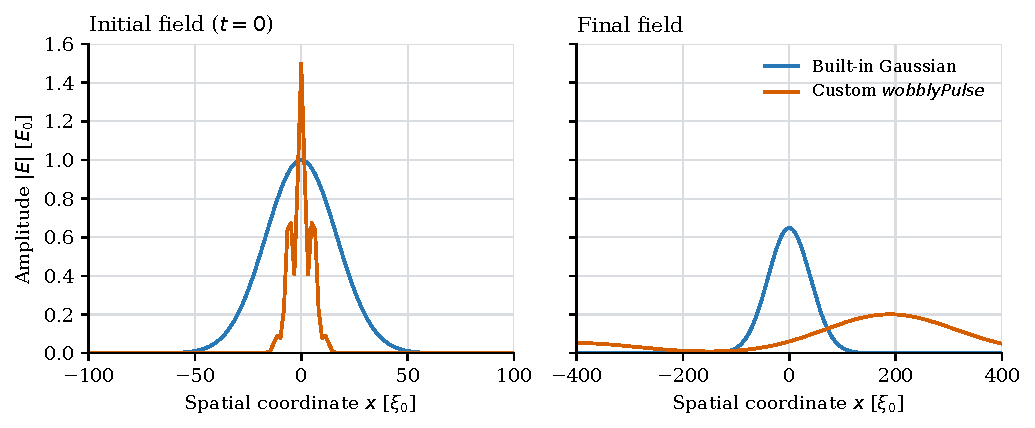
\includegraphics[width=0.9\textwidth]{simulation_builtin_vs_custom}
  \caption{Initial (left) and final (right) field amplitudes for the built-in Gaussian and
  custom pulse, launched as two forward channels in one simulation. The Gaussian's initial
  profile is the same as in \cref{fig:simulation-gaussian-evolution}. The horizontal ranges
  differ to show the full profiles before and after propagation.}
  \label{fig:simulation-builtin-custom}
\end{figure}

% Plan: ~2 pages.
\section{Performance Benchmarking}

The first performance experiments isolated the linear propagation path by disabling all
nonlinear effects. The linear computation was the first part ported to using \texttt{FieldData}
objects, and hence benchmarking acted as a proof of concept. The experiments compared the
Eigen CPU implementation with LibTorch on the GPU while varying the number of spatial grid
points and optical channels.

\Cref{fig:linear-grid-sweep} shows total simulation time for one optical channel as the grid
size increases. At the smallest measured grid size, the GPU was slower than the CPU (a
CPU-to-GPU time ratio of 0.5). The GPU became faster as the problem grew: the ratio reached
6.6 at 131,072 grid points and 18.6 at 1,048,576 grid points. Below grid sizes of $2^{15}$, 
the cost of launching a GPU operation becomes the main cost in time, and the actual operations 
don't become any faster, so the CPU is able to be quicker in those situations. In practice,
grid points would be kept above this level for higher precision, and the GPU advantage would 
be relevant.

\begin{figure}
  \centering
  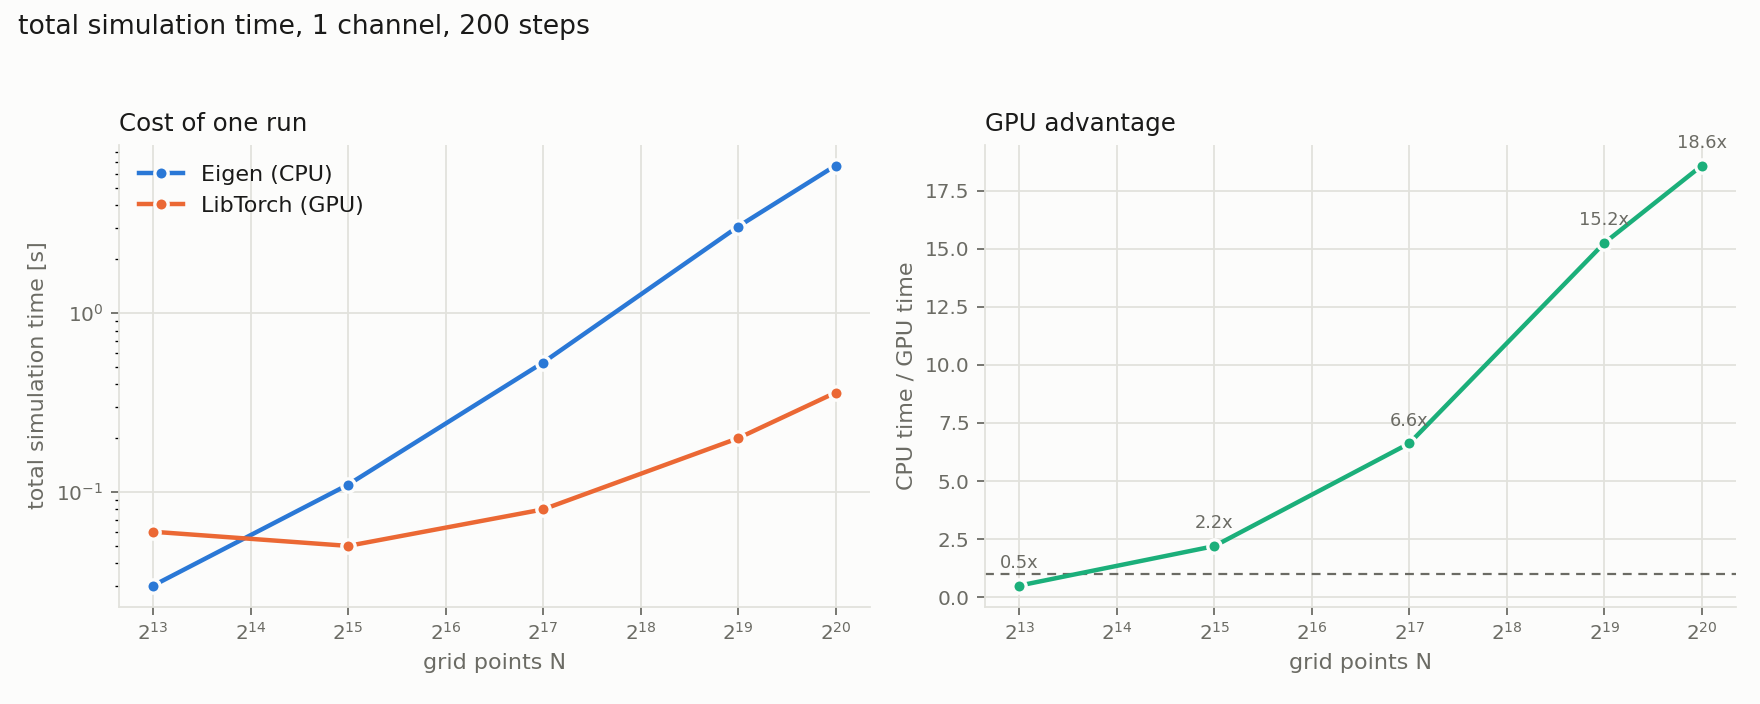
\includegraphics[width=\textwidth]{Figure linear only - Sweeping grid points}
  \caption{Linear-only simulation time and CPU-to-GPU speedup while sweeping the number of
  grid points. The simulation uses one optical channel and 200 propagation steps.}
  \label{fig:linear-grid-sweep}
\end{figure}

The channel-count sweep in \cref{fig:linear-channel-sweep} holds the grid size at 131,072
points and uses 200 propagation steps. The measured GPU speedup ranged from 7.7 for one
channel to 19.9 for 128 channels. This increase is consistent with the GPU using its parallel
compute resources more effectively as more field data is processed. Together, the two sweeps
show that the linear-only GPU implementation benefits from larger grids and more channels,
although the size sweep shows that a GPU is not necessarily faster for small problems.

\begin{figure}
  \centering
  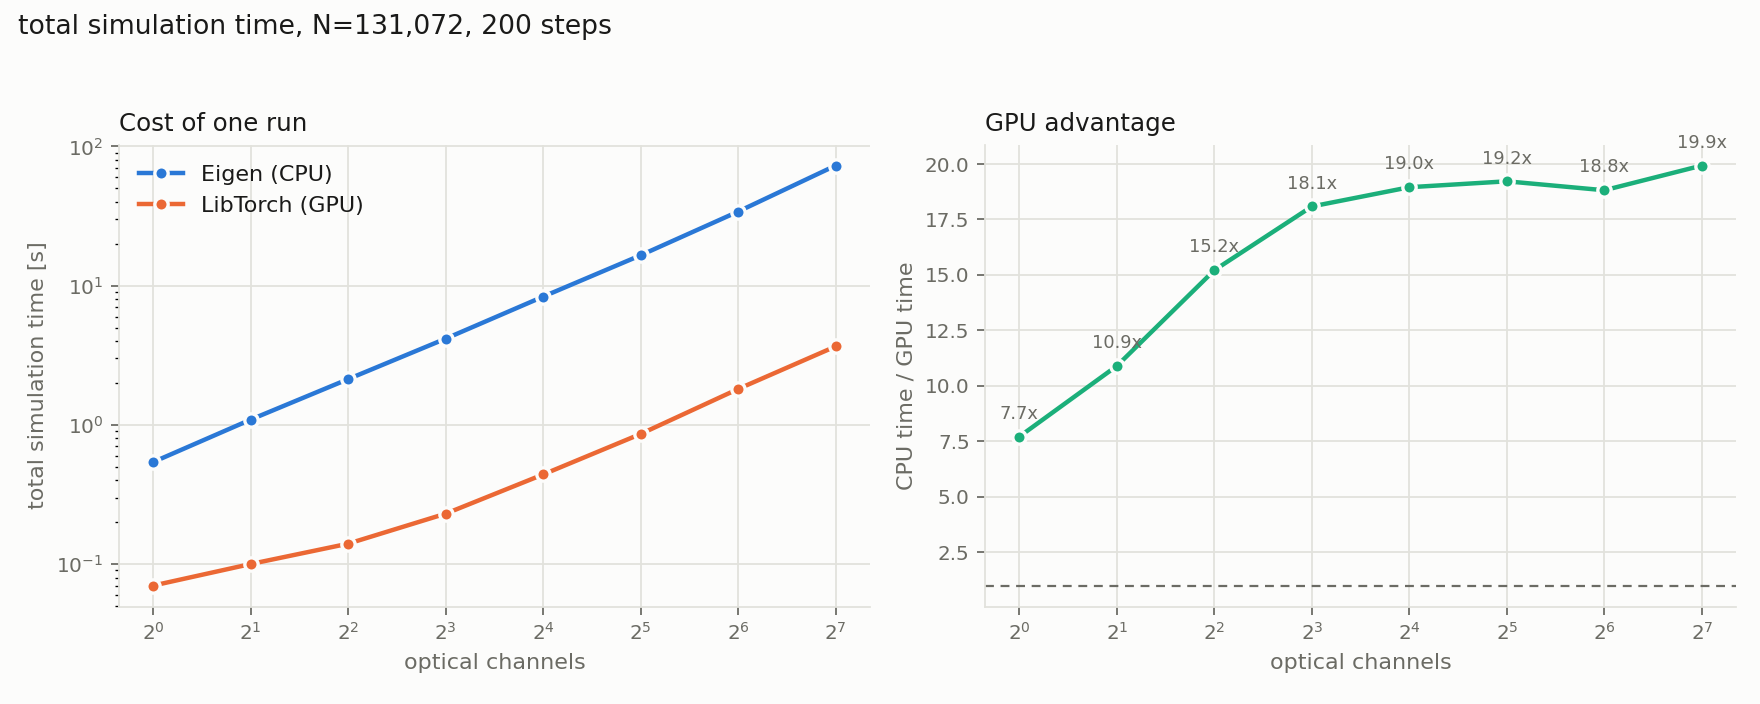
\includegraphics[width=\textwidth]{Figure linear only - sweeping optial channels}
  \caption{Linear-only simulation time and CPU-to-GPU speedup while sweeping the number of
  optical channels. The grid contains 131,072 points and the simulation uses 200 propagation
  steps.}
  \label{fig:linear-channel-sweep}
\end{figure}

Once the nonlinear effects were able to run across both backings through \texttt{FieldData} objects, 
the next experiment enabled nonlinear effects in addition to the linear propagation terms.
This tests whether the performance trend in the linear-only case also holds when the
nonlinear calculation is included, and provides comparison between GPU and CPU speed for the program
as a whole. As mentioned before, grid sizes below $2^{15}$ have their timing dominated by kernel launches
and that explains why they are seen as unusually slow in the right graph of \Cref{fig:four-channel-nonlinear-speed}.

\begin{figure}
  \centering
  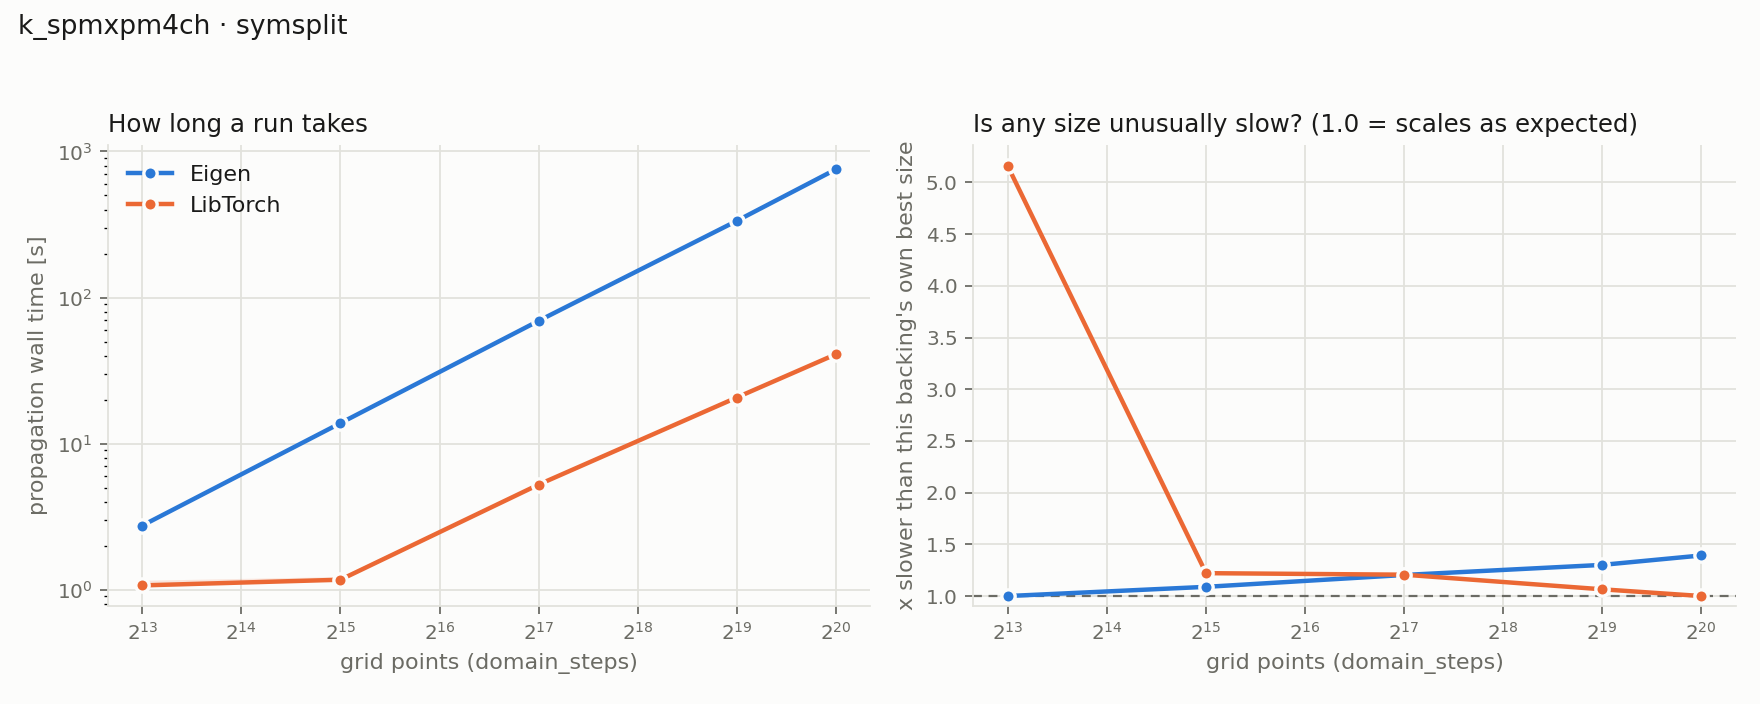
\includegraphics[width=\textwidth]{speed_k_spmxpm4ch_symsplit}
  \caption{Propagation time for the symmetric split-step method with SPM and XPM enabled
  across four optical channels. The left panel shows runtime as grid size increases; the right
  panel compares scaling against each backing's own best result.}
  \label{fig:four-channel-nonlinear-speed}
\end{figure}

\begin{figure}
  \centering
  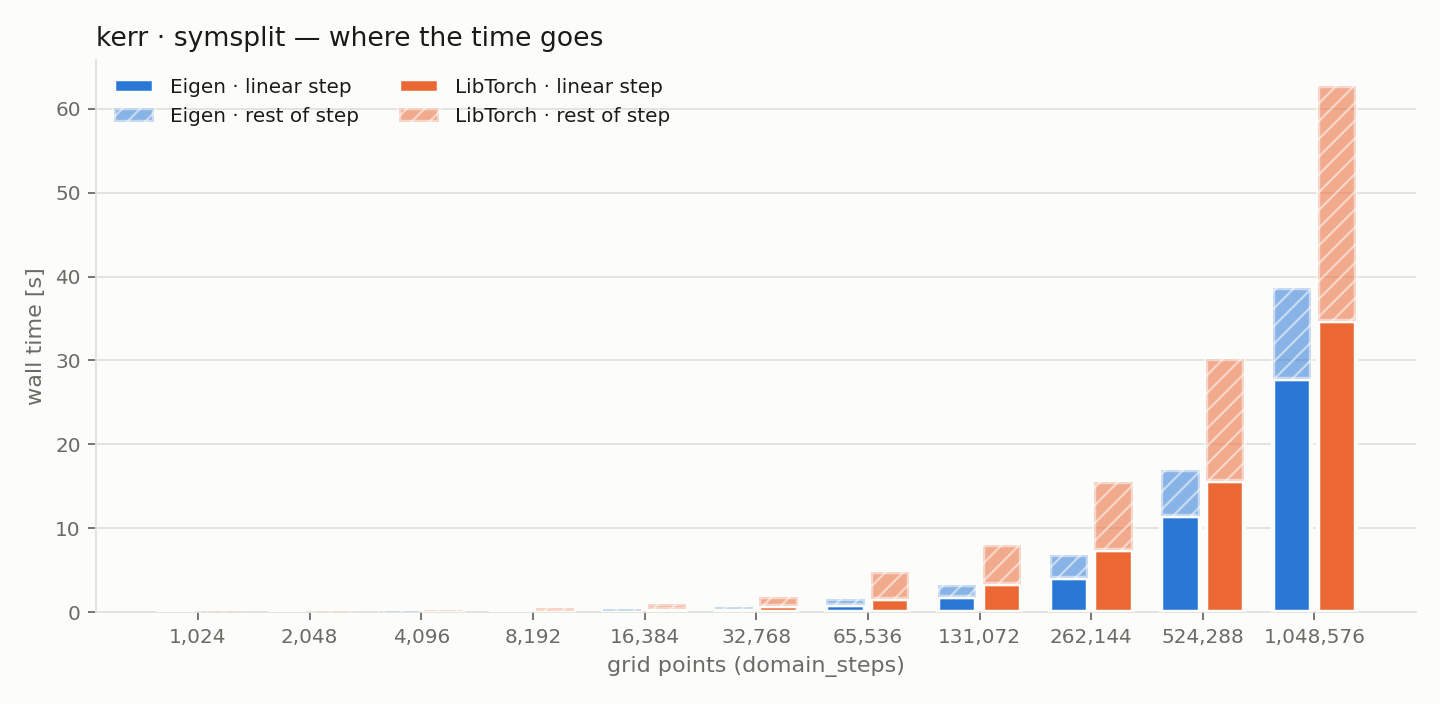
\includegraphics[width=\textwidth]{split_kerr_symsplit}
  \caption{Time spent in the linear step and the remaining work for the Kerr benchmark using
  symmetric split-step. The remaining-work segment includes the nonlinear calculation and
  time outside the measured linear step.}
  \label{fig:kerr-time-split}
\end{figure}

\subsection{Which Parts of the Simulation Take the Most Time?}

The timing breakdown in \Cref{fig:kerr-time-split} compares the linear step with the
remaining work in the simulation. The benchmarks show that the linear part receives a
greater performance improvement from GPU execution than the nonlinear part. This difference
is related to how each part processes the field data (\texttt{svea}). In one SPM-only step,
the nonlinear calculation performs 39 operations and reads or writes \texttt{svea} 84
times. The linear calculation performs 6 operations and reads or writes \texttt{svea} 15
times. The repeated field-data accesses in the nonlinear calculation create more memory
traffic and more intermediate operations, which limits the performance improvement it gets
from the GPU. By comparison, the linear calculation consists largely of FFT operations,
which are well suited to GPU execution. The operation counts provide a simple explanation
for the difference, although the exact performance improvement depends on the hardware and
simulation configuration.

\subsection{Precision and loss effects}

The LibTorch results above use double-precision complex values, matching that of Eigen. 
The FP64 ratio (64 bit floating-point ratio) refers to the throughput ratio of FP64 arithmetic on a GPU
compared to FP32 (32 bit floating-point) arithmetic. Typical consumer GPU cards have an FP64 ratio of 1:64,
meaning that double-precision operations take 64 times as long to be performed.
Common high-end GPUs in HPC can have FP64 ratio as good as 1:2, such as the NVIDIA V100, A100, or H100.
Since double-precision arithmetic can be substantially more expensive on some GPUs than single-precision arithmetic,
a further experiment compares LibTorch performance using 64-bit and 32-bit floating-point
values. The measured runtimes are shown in \Cref{tab:precision-speedup}. Across the tested
grid sizes, single precision was approximately 2.4--2.5 times faster than double precision.
This is however specific to the hardware used; in the following precision comparison, it was a 
Tesla T4 GPU with a FP64 ratio of 1:32.

\begin{table}[H]
  \centering
  \caption{Runtime and speedup for single and double-precision LibTorch simulations on a
  Tesla T4 GPU. The speedup is the double-precision runtime divided by the single-precision
  runtime.}
  \label{tab:precision-speedup}
  \begin{tabular}{rrrrrr}
    \toprule
    $N$ & Double (s) & Float (s) & Speedup & Linear speedup & nonlinear speedup \\
    \midrule
    $2^{20}$ & 9.4 & 3.9 & 2.4$\times$ & 4.1$\times$ & 2.0$\times$ \\
    $2^{21}$ & 18.1 & 7.4 & 2.4$\times$ & 4.1$\times$ & 2.0$\times$ \\
    $2^{22}$ & 36.3 & 14.8 & 2.5$\times$ & 4.2$\times$ & 2.0$\times$ \\
    \bottomrule
  \end{tabular}
\end{table}

The precision comparison introduces a measurable accuracy cost, summarised in
\Cref{tab:precision-error}. The maximum field difference is measured relative to the peak
of the double-precision field. After 1,000 steps the difference remains small, but it grows
substantially after 10,000 steps. The float run also loses energy, with greater loss over the
longer run.

\begin{table}[H]
  \centering
  \caption{Difference and energy change for single-precision LibTorch relative to
  double-precision LibTorch on a Tesla T4, using the symmetric split-step method with
  $N=2^{20}$. The maximum field error is normalised by the peak of the double-precision
  field.}
  \label{tab:precision-error}
  \begin{tabular}{rrr}
    \toprule
    Steps & Maximum field error / peak & Energy change (float) \\
    \midrule
    1,000 & $5.1\times10^{-4}$ & $-0.043\%$ \\
    10,000 & $5.2\times10^{-2}$ & $-0.44\%$ \\
    \bottomrule
  \end{tabular}
\end{table}

An additional dispersion-only test and a direct FFT round-trip test help identify the source
of this energy loss. With nonlinear effects disabled, 1,000 single-precision steps produced
an energy change of $-4.3\times10^{-4}$. Applying 1,000 forward and inverse complex64 FFT
round trips to a field of size $2^{20}$ produced a similar change ($-4.25\times10^{-4}$),
whereas complex128 changed the energy by approximately $4\times10^{-13}$. This indicates
that the observed loss is associated with single-precision FFT round-off in cuFFT rather
than the propagation phase itself. Repeated small downward changes can accumulate over many
steps. The separate error-growth test at 8,192 points shows that the maximum field error
grows approximately linearly with step count when Kerr is disabled, and approximately
quadratically when Kerr is enabled over the measured range. The Kerr-enabled curve follows
the plotted slope-two guide, while the dispersion-only curve grows more slowly. This supports
the interpretation that nonlinear effects compound the numerical differences; these growth
rates describe the tested configuration and range.

\subsection{Summary}

The measurements show that GPU acceleration is most useful once the workload is sufficiently
large. With four channels and SPM/XPM enabled, the GPU also outperformed the CPU for the
tested grid sizes. The timing breakdown shows that the linear and remaining parts of the
simulation contribute differently to total runtime. Although using single precision gave an
approximately 2.4-fold speedup over double precision for the tested grid sizes, the error in
the results makes it unusable past generating a quick answer where exact precision isn't required.
The exact results are specific to the tested hardware and configurations.
